\PassOptionsToPackage{unicode=true}{hyperref} % options for packages loaded elsewhere
\PassOptionsToPackage{hyphens}{url}
\documentclass[9pt,ignorenonframetext,aspectratio=169]{beamer}
\IfFileExists{pgfpages.sty}{\usepackage{pgfpages}}{}
\setbeamertemplate{caption}[numbered]
\setbeamertemplate{caption label separator}{: }
\setbeamercolor{caption name}{fg=normal text.fg}
\beamertemplatenavigationsymbolsempty
\usepackage{lmodern}
\usepackage{amssymb,amsmath}
\usepackage{ifxetex,ifluatex}
\usepackage{fixltx2e} % provides \textsubscript
\ifnum 0\ifxetex 1\fi\ifluatex 1\fi=0 % if pdftex
  \usepackage[T1]{fontenc}
  \usepackage[utf8]{inputenc}
\else % if luatex or xelatex
  \ifxetex
    \usepackage{mathspec}
  \else
    \usepackage{fontspec}
\fi
\defaultfontfeatures{Ligatures=TeX,Scale=MatchLowercase}







\fi

  \usetheme[]{metropolis}






% use upquote if available, for straight quotes in verbatim environments
\IfFileExists{upquote.sty}{\usepackage{upquote}}{}
% use microtype if available
\IfFileExists{microtype.sty}{%
  \usepackage{microtype}
  \UseMicrotypeSet[protrusion]{basicmath} % disable protrusion for tt fonts
}{}


\newif\ifbibliography
  \usepackage[style=abnt,]{biblatex}
      \addbibresource{references.bib}
  

\hypersetup{
      pdftitle={Modelos mistos na Engenharia de Avaliações},
        pdfauthor={Luiz Fernando Palin Droubi ; Carlos Augusto Zilli ; Norberto Hochheim},
          pdfborder={0 0 0},
    breaklinks=true}
%\urlstyle{same}  % Use monospace font for urls







% Prevent slide breaks in the middle of a paragraph:
\widowpenalties 1 10000
\raggedbottom

  \AtBeginPart{
    \let\insertpartnumber\relax
    \let\partname\relax
    \frame{\partpage}
  }
  \AtBeginSection{
    \ifbibliography
    \else
      \let\insertsectionnumber\relax
      \let\sectionname\relax
      \frame{\sectionpage}
    \fi
  }
  \AtBeginSubsection{
    \let\insertsubsectionnumber\relax
    \let\subsectionname\relax
    \frame{\subsectionpage}
  }



\setlength{\parindent}{0pt}
\setlength{\parskip}{6pt plus 2pt minus 1pt}
\setlength{\emergencystretch}{3em}  % prevent overfull lines
\providecommand{\tightlist}{%
  \setlength{\itemsep}{0pt}\setlength{\parskip}{0pt}}

  \setcounter{secnumdepth}{0}


  \usepackage[brazil]{babel}
  \usepackage{animate}

  \title[]{Modelos mistos na Engenharia de Avaliações}

  \subtitle{Possibilidades e aplicações}

  \author[
        Luiz Fernando Palin Droubi\footnote<.->{\href{mailto:lfpdroubi@gmail.com}{\nolinkurl{lfpdroubi@gmail.com}}}
\newline \and Carlos Augusto Zilli\footnote<.->{\href{mailto:carlos.zilli@ifsc.edu.br}{\nolinkurl{carlos.zilli@ifsc.edu.br}}}
\newline \and Norberto Hochheim\footnote<.->{\href{mailto:norberto.hochheim@ufsc.br}{\nolinkurl{norberto.hochheim@ufsc.br}}}
    ]{Luiz Fernando Palin Droubi\footnote<.->{\href{mailto:lfpdroubi@gmail.com}{\nolinkurl{lfpdroubi@gmail.com}}}
\newline \and Carlos Augusto Zilli\footnote<.->{\href{mailto:carlos.zilli@ifsc.edu.br}{\nolinkurl{carlos.zilli@ifsc.edu.br}}}
\newline \and Norberto Hochheim\footnote<.->{\href{mailto:norberto.hochheim@ufsc.br}{\nolinkurl{norberto.hochheim@ufsc.br}}}}

  \institute[
    ]{
    GEAP - UFSC
    }

\date[
      \today
  ]{
      \today
        }


\begin{document}

% Hide progress bar and footline on titlepage
  \begin{frame}[plain]
  \titlepage
  \end{frame}


  \begin{frame}
  \tableofcontents[hideallsubsections]
  \end{frame}

\hypertarget{introduuxe7uxe3o}{%
\section{Introdução}\label{introduuxe7uxe3o}}

\begin{frame}{Amostras heterogêneas}
\protect\hypertarget{amostras-heteroguxeaneas}{}

\begin{itemize}[<+->]
\tightlist
\item
  \alert<1>{Modelos mistos são modelos estatísticos que misturam efeitos fixos 
  (FE) e efeitos aleatórios (RE), capazes de lidar com a heterogeneidade amostral 
  \footcite{bell2019}.}

  \begin{itemize}[<+->]
  \tightlist
  \item
    \alert<2>{\begin{equation}
    y_{ij} = \beta_0 + \beta_1^{RE} x_{ij} + \beta_2 z_j + (\upsilon_j + \varepsilon_{ij})
    \end{equation}}
  \item
    \alert<3>{$\upsilon_j \sim \mathcal N(0, \sigma^2_{\upsilon})$ e 
    $\varepsilon_{ij} \sim \mathcal N(0, \sigma^2_{\varepsilon})$}
  \end{itemize}
\end{itemize}

\begin{itemize}[<+->]
\tightlist
\item
  \alert<4>{Existem outras maneiras de modelar amostras heterogêneas}

  \begin{itemize}[<+->]
  \tightlist
  \item
    \alert<5>{Modelos de Efeitos Fixos (FE): variância entre agrupamentos $\infty$}

    \begin{itemize}[<+->]
    \tightlist
    \item
      \alert<6>{\begin{equation}
      y_{ij} = \sum_{j=1}^{j}\beta_{0j}D_j + \beta_1 x_{ij} + \varepsilon_{ij}
      \end{equation}}
    \end{itemize}
  \item
    \alert<7>{Modelos OLS: ignorar a heterogeneidade}

    \begin{itemize}[<+->]
    \tightlist
    \item
      \alert<8>{\begin{equation}
      y_{ij} = \beta_0 + \beta_1^{OLS} x_{ij} + \beta_2 z_j + \varepsilon_{ij}
      \end{equation}}
    \item
      \alert<9>{Pode levar a não verificação de várias hipóteses da 
      inferência clássica, como a independência das observações.}
    \end{itemize}
  \end{itemize}
\end{itemize}

\end{frame}

\begin{frame}{Efeitos Fixos vs.~Efeitos Aleatórios}
\protect\hypertarget{efeitos-fixos-vs.-efeitos-aleatuxf3rios}{}

\begin{itemize}[<+->]
\tightlist
\item
  \alert<1>{A utilização de uma ou outra abordagem vai depender do objetivo da
  modelagem e da composição da amostra.}
\item
  \alert<2>{Na avaliação de precisão de um imóvel em específico, a partir de
  uma amostra heterogênea, com dados de poucos agrupamentos, onde não haja
  interesse em \emph{explicar} porque os dados de um agrupamento apresentam
  valores diferentes, em média, dos dados de outros agrupamentos.}

  \begin{itemize}[<+->]
  \tightlist
  \item
    \alert<3>{O modelo de efeitos fixos é ideal.}
  \item
    \alert<4>{Um número mínimo de dados em cada agrupamento, no entanto, é
    necessário para uma boa estimação.}
  \end{itemize}
\end{itemize}

\begin{itemize}[<+->]
\tightlist
\item
  \alert<5>{Na elaboração de PVGs, onde estão disponíveis dados em uma grande
  quantidade de agrupamentos (não necessariamente todos), porém seja necessária a 
  previsão de valores em agrupamentos fora da amostra.}

  \begin{itemize}[<+->]
  \tightlist
  \item
    \alert<6>{O modelo de efeitos aleatórios deve ser utilizado, já que a 
    modelagem por efeitos fixos não pode \emph{explicar} a diferença de níveis entre 
    os agrupamentos, impossibilitando a previsão de valores em agrupamentos fora da
    amostra.}
  \item
    \alert<7>{Estimação em agrupamentos com pequeno $n_j$ é beneficiada pelo 
    efeito do encolhimento (\emph{borrowing strenght}\footcite[p. 196]{tukey}).}
  \end{itemize}
\end{itemize}

\end{frame}

\begin{frame}{Modelagem hierárquica}
\protect\hypertarget{modelagem-hieruxe1rquica}{}

\begin{itemize}[<+->]
\tightlist
\item
  \alert<1>{Modelos hierárquicos ou multiníveis são modelos cujas equações 
  podem ser escritas separadamente, dividindo a modelagem em diversos níveis de
  análise.}
\item
  \alert<2>{Apesar do modelo ser escrito em diversos níveis, a estimação é feita
  de uma só vez, a partir da substituição das equações}

  \begin{itemize}[<+->]
  \tightlist
  \item
    \alert<3>{P. Ex.: 
    \begin{align}
    y_{ij} &= \beta_{0j} + \beta_1^{RE}x_{ij} + \varepsilon_{ij}\\
    \beta_{0j} &= \beta_0 + \beta_2 z_j + \upsilon_j \\
    y_{ij} &= \beta_0 + \beta_1^{RE} x_{ij} + \beta_2 z_j + (\upsilon_j + \varepsilon_{ij})
    \end{align}
    }
  \end{itemize}
\item
  \alert<4>{Possibilidade de modelagem de diversos níveis aninhados.}
\item
  \alert<5>{Todo modelo hierárquico é um modelo misto.}
\item
  \alert<6>{Nem todo modelo misto é um modelo hierárquico.}
\end{itemize}

\end{frame}

\hypertarget{inclinauxe7uxf5es-aleatuxf3rias}{%
\section{Inclinações Aleatórias}\label{inclinauxe7uxf5es-aleatuxf3rias}}

\begin{frame}{Inclinações Aleatórias}

\begin{itemize}[<+->]
\tightlist
\item
  \alert<1>{Os modelos mistos são mais flexíveis que os modelos fixos.}
\item
  \alert<2>{É fácil introduzir inclinações aleatórias, p. ex.}

  \begin{itemize}[<+->]
  \tightlist
  \item
    \alert<3>{\begin{equation}
    y_{ij} = (\beta_0 + \upsilon_j) + (\beta_1 + \nu_j) x_{ij} + \beta_2 z_j + \varepsilon_{ij}
    \end{equation}}
  \item
    \alert<4>{Apenas um grau de liberdade a mais é consumido}
  \end{itemize}
\item
  \alert<5>{Para obtenção de uma modelagem análoga com a abordagem de efeitos fixos, seria necessário modelar a interação entre as variáveis \emph{dummies} e 
  a variável com inclinações aleatórias.}
\item
  \alert<6>{Processo é custoso em graus de liberdade e pode prejudicar uma boa
  estimação dos coeficientes.}
\end{itemize}

\end{frame}

\begin{frame}{Encolhimento (borrowing strenght)}
\protect\hypertarget{encolhimento-borrowing-strenght}{}

\begin{figure}

{\centering 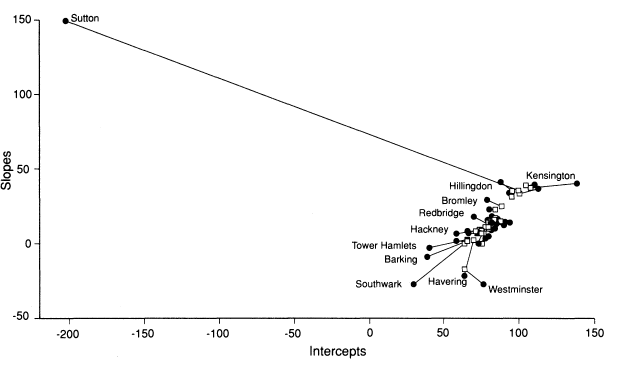
\includegraphics[width=0.7\linewidth]{../../images/shrinkage} 

}

\caption{Encolhimento em modelos mistos \footcite{jones1994}.}\label{fig:unnamed-chunk-1}
\end{figure}

\end{frame}

\begin{frame}{Encolhimento (borrowing strenght) (2)}
\protect\hypertarget{encolhimento-borrowing-strenght-2}{}

\begin{figure}

{\centering 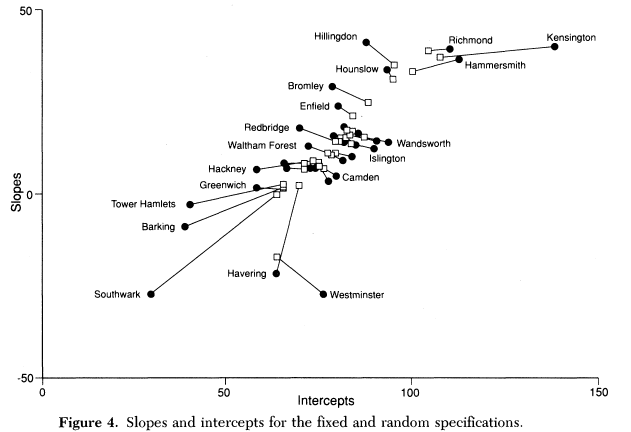
\includegraphics[width=0.7\linewidth]{../../images/shrinkage2} 

}

\caption{Encolhimento em modelos mistos (2) \footcite{jones1994}.}\label{fig:unnamed-chunk-2}
\end{figure}

\end{frame}

\begin{frame}{Encolhimento (borrowing strenght) (3)}
\protect\hypertarget{encolhimento-borrowing-strenght-3}{}

\begin{center}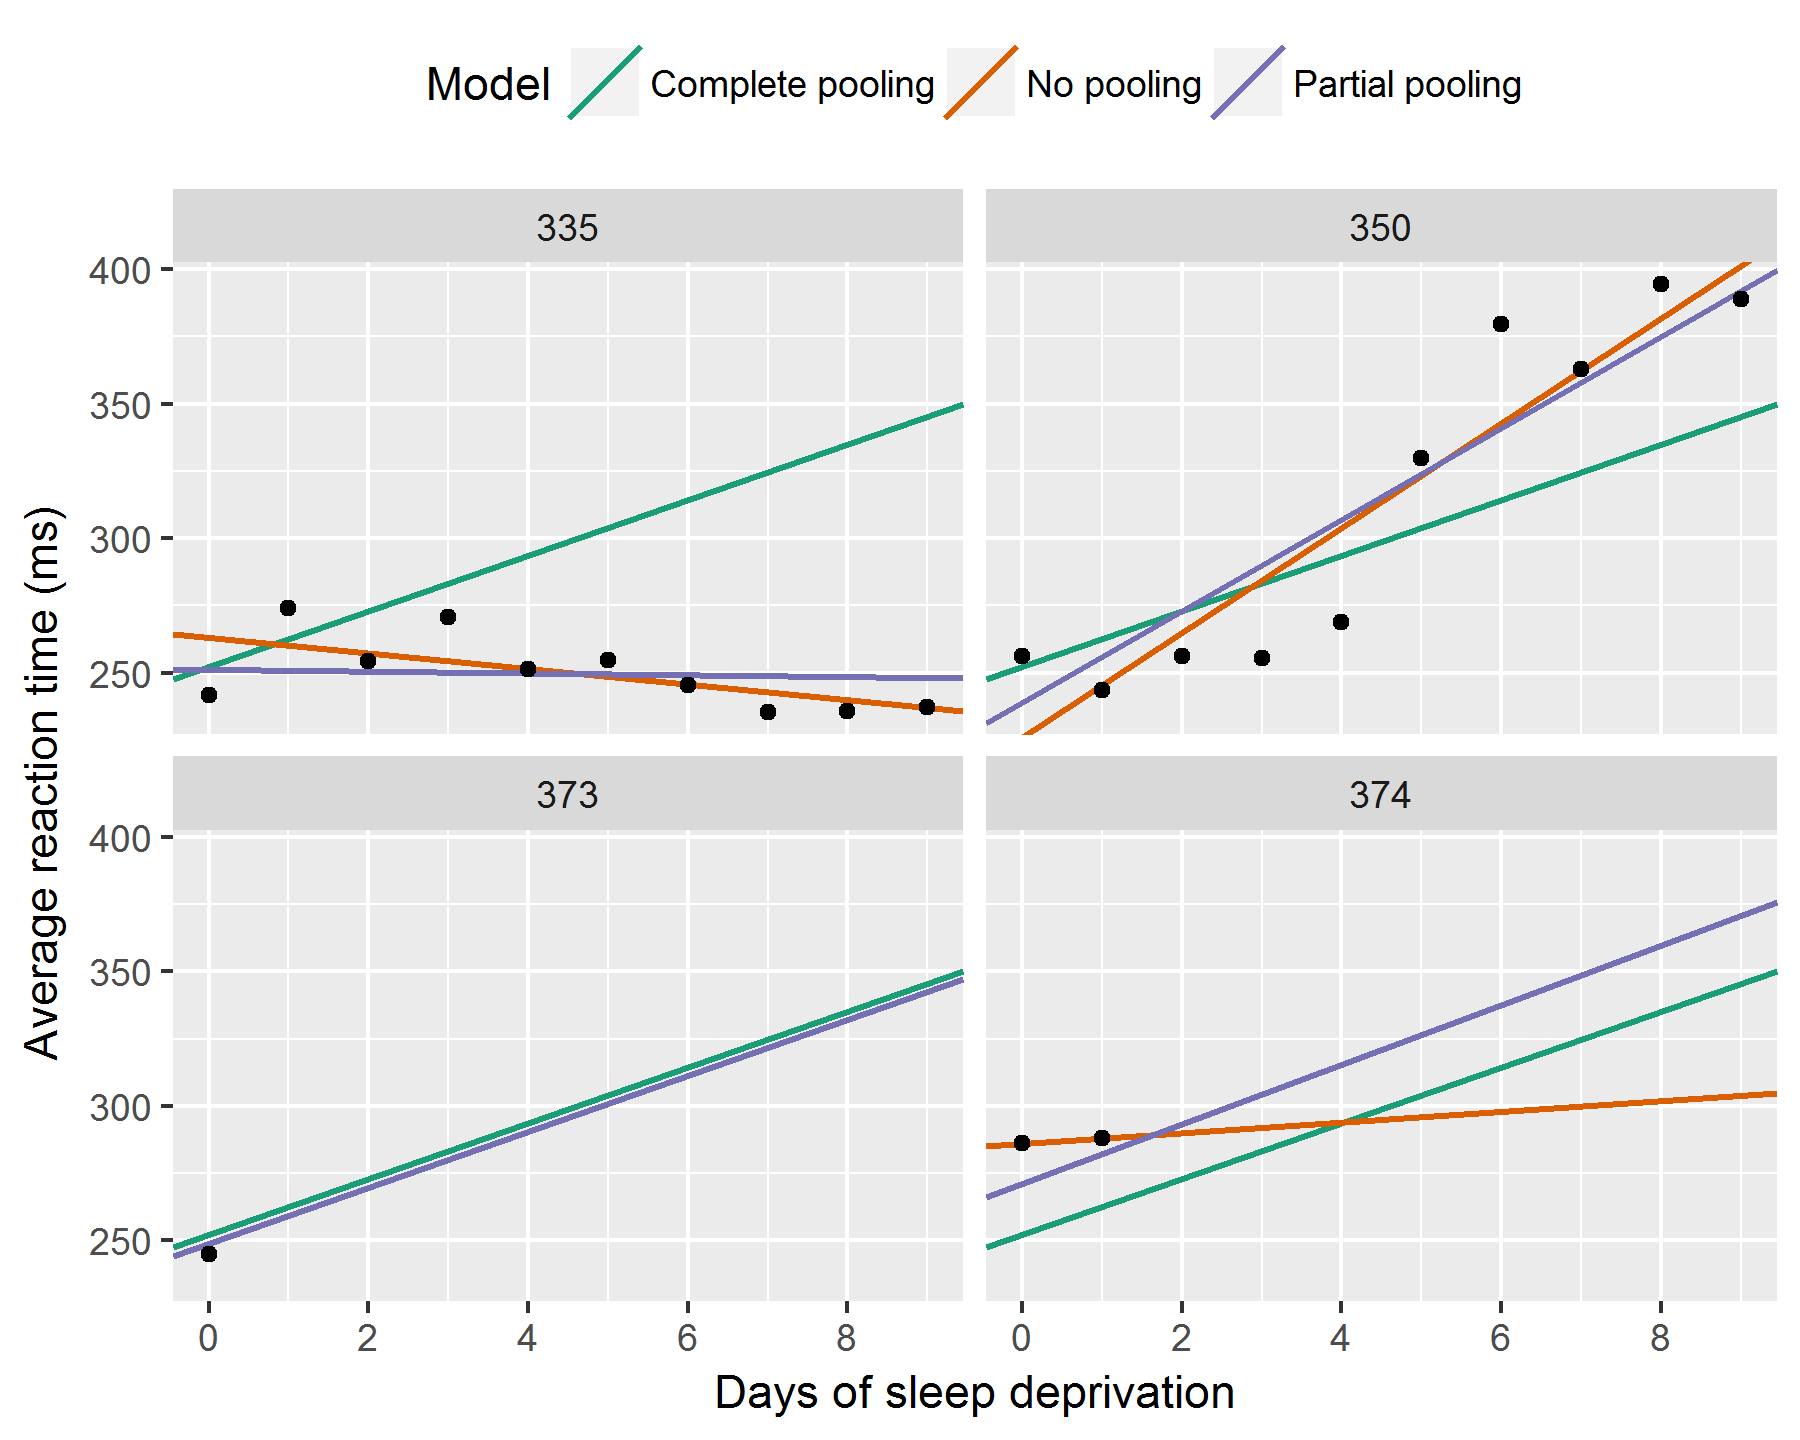
\includegraphics[width=0.5\linewidth]{../../images/zoomed-in-partial-pooling} \end{center}

\end{frame}

\hypertarget{limitauxe7uxf5es-e-outras-formulauxe7uxf5es}{%
\section{Limitações e outras
formulações}\label{limitauxe7uxf5es-e-outras-formulauxe7uxf5es}}

\begin{frame}{Limitações e outras formulações}

\begin{itemize}[<+->]
\tightlist
\item
  \alert<1>{A formação de efeitos aleatórios supõe que \footcite[p. 138]{bell2015}:}

  \begin{itemize}[<+->]
  \tightlist
  \item
    \alert<2>{$Cov(x_{ij}; u_j) = 0$ e $Cov(x_{ij}; e_{ij}) = 0$}
  \end{itemize}
\item
  \alert<3>{Estas hipóteses frequentemente não se verificam$^4$.}
\item
  \alert<4>{No entanto, é possível contornar este problema:}

  \begin{itemize}[<+->]
  \tightlist
  \item
    \alert<5>{Formulação de Mundlak \footcite[p. 141]{bell2015}:
    \begin{align}
    y_{ij} &= \beta_{0j} + \beta_1^{RE}x_{ij} + \varepsilon_{ij}\\
    \beta_{0j} &= \beta_0 + \beta_2 z_j + \beta_3 \bar x_{ij} + \upsilon_j 
    \end{align}
    }
  \item
    \alert<6>{Formulação REWB$^5$:
    \begin{align}
    y_{ij} &= \beta_{0j} + \beta_1^{RE}x_{ij} + \varepsilon_{ij}\\
    \beta_{0j} &= \beta_0 + \beta_2 z_j + (\beta_4 - \beta_1) \bar x_{ij} + \upsilon_j\\ 
    y_{ij} &= \beta_0 + \beta_1 (x_{ij} - \bar x_j) + \beta_4 \bar x_{ij} + \beta_2 z_j + (\upsilon_j + \varepsilon_{ij})
    \end{align}
    }
  \end{itemize}
\end{itemize}

\end{frame}

\hypertarget{estudo-de-caso}{%
\section{Estudo de Caso}\label{estudo-de-caso}}

\begin{frame}{Criação dos dados}
\protect\hypertarget{criauxe7uxe3o-dos-dados}{}

\begin{align}
ValorUnitario &= \beta_{0j} - 3,0 \cdot Area + \varepsilon_{ij}  \label{eq:EC1}\\
\beta_{0j} &= 3000 + 4000 \cdot A_{Vj} + 5,0 \cdot \overline{Area_j} + \upsilon_j \label{eq:EC2}
\end{align}

\begin{figure}

{\centering 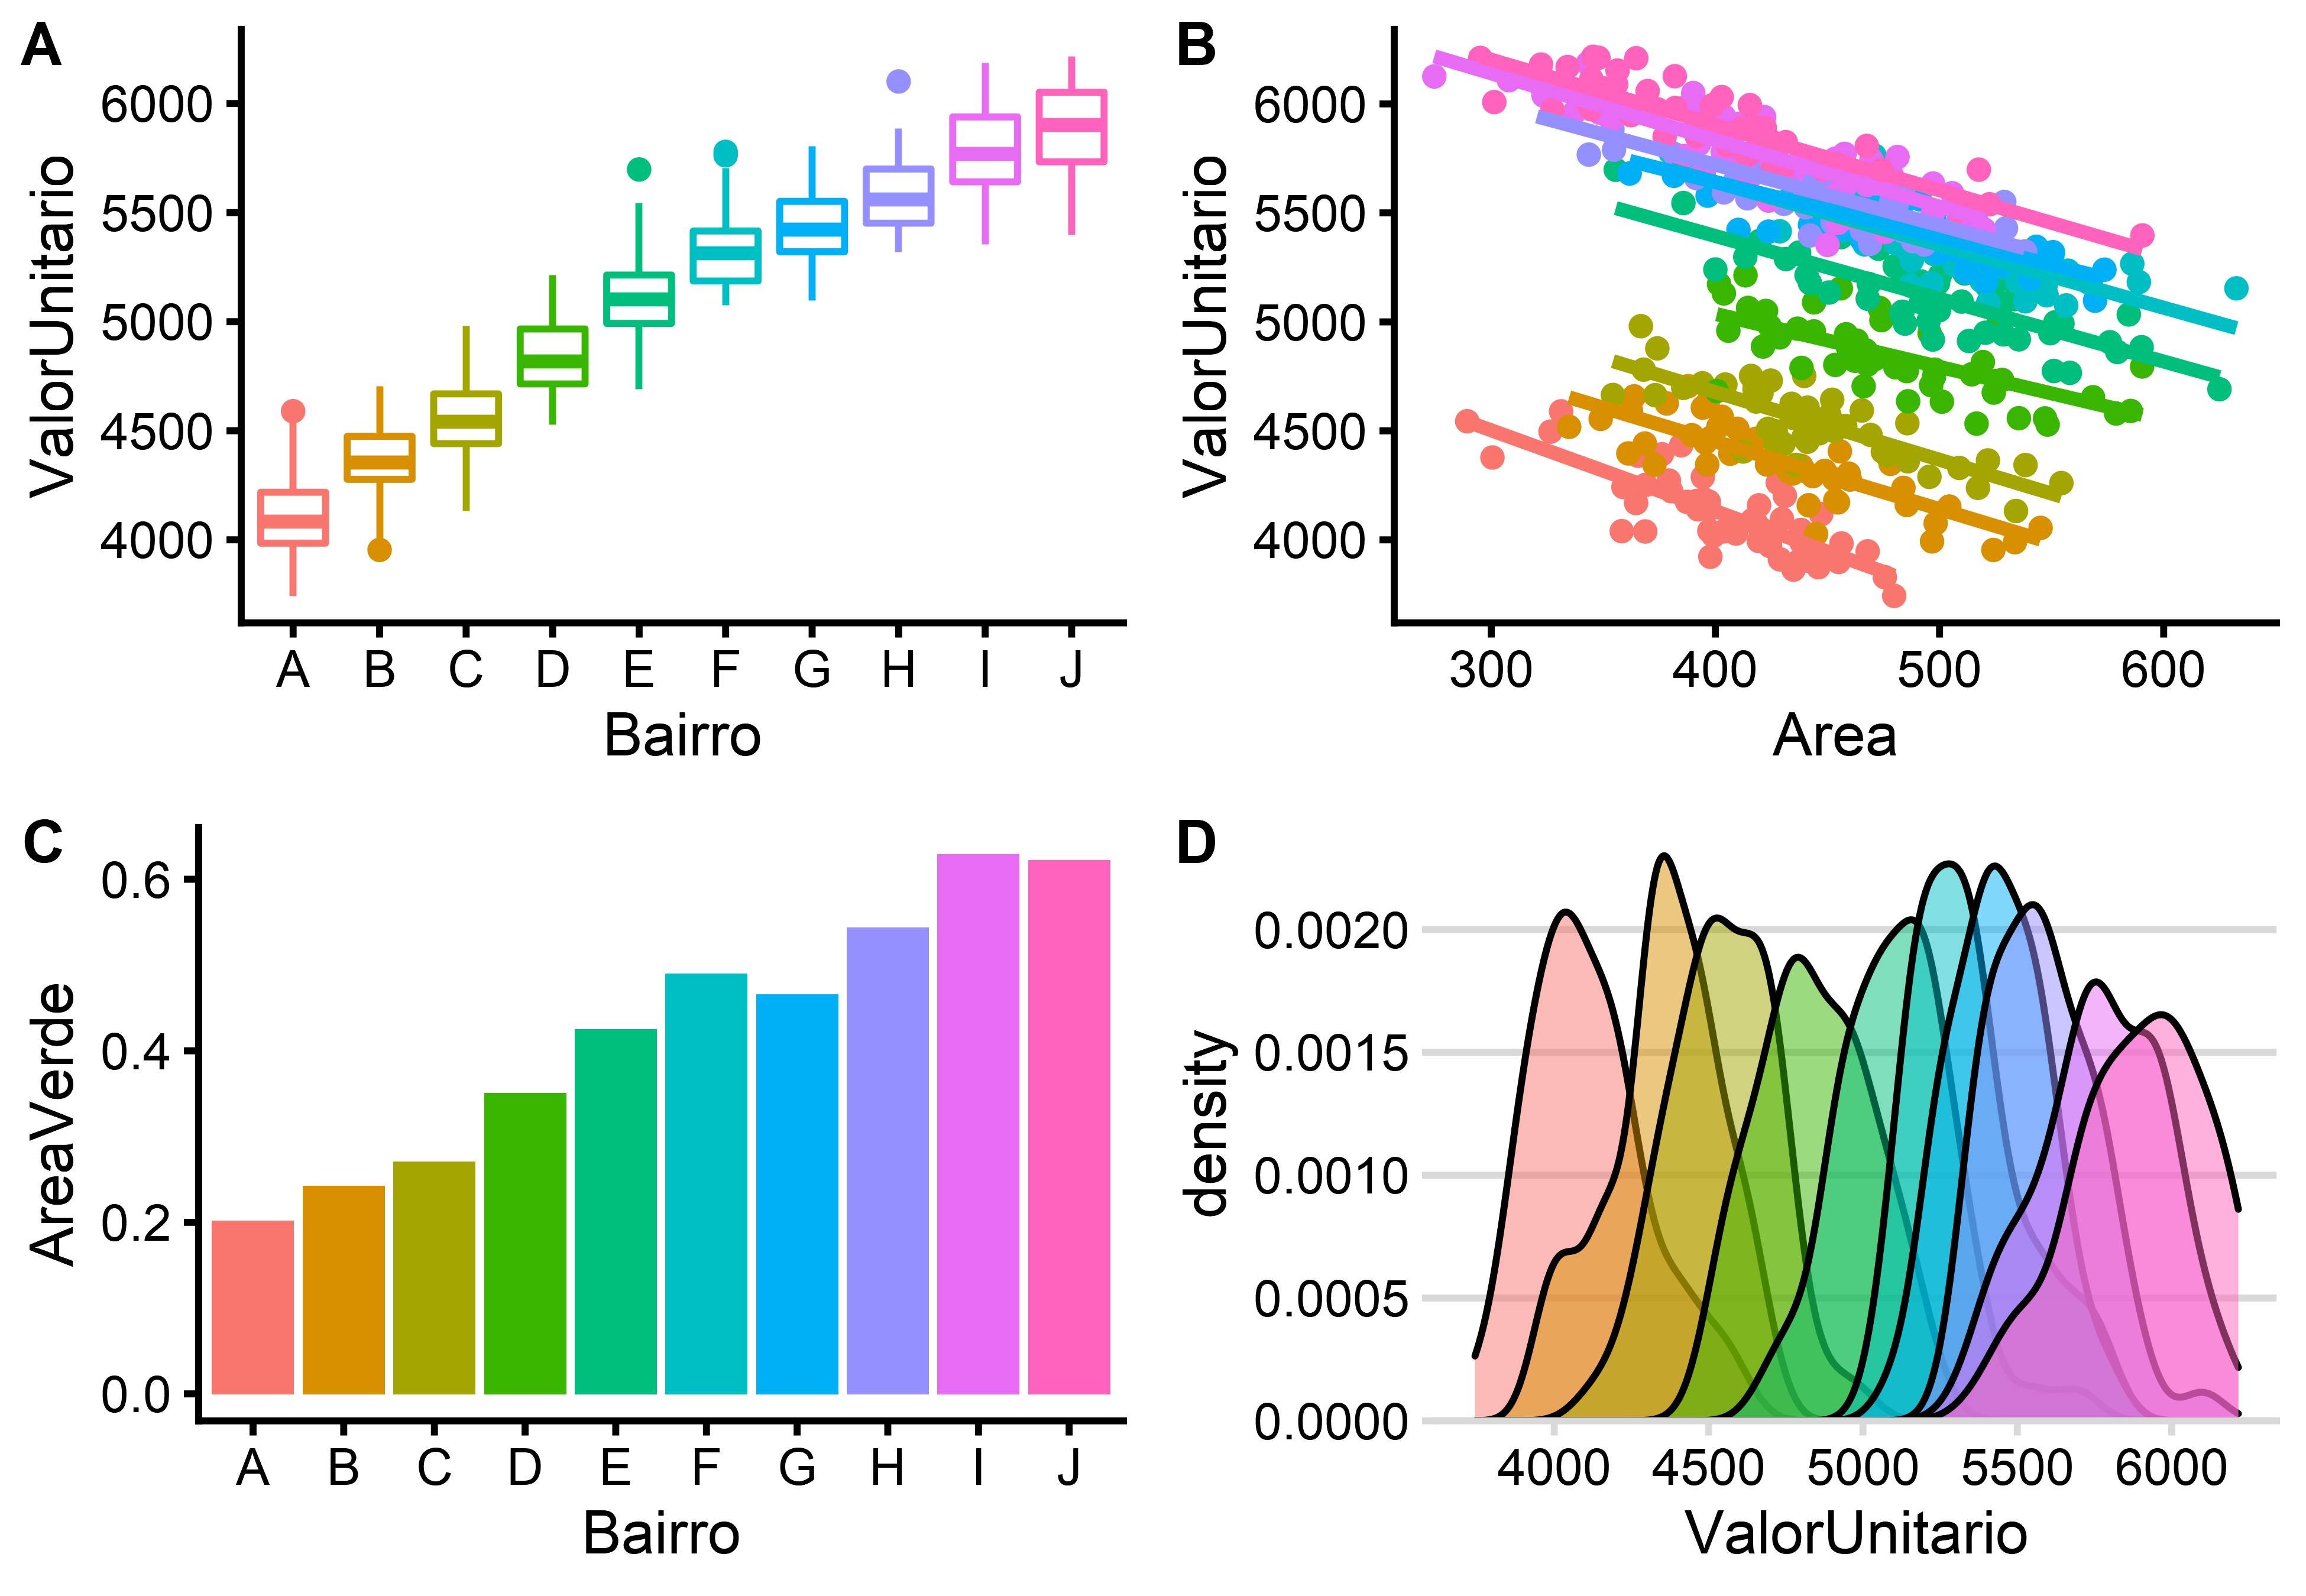
\includegraphics[width=0.5\linewidth]{../../images/exploratoria-1} 

}

\caption{Dados simulados. Fonte: Os autores}\label{fig:unnamed-chunk-4}
\end{figure}

\end{frame}

\begin{frame}{Ajuste de modelos}
\protect\hypertarget{ajuste-de-modelos}{}

\begin{itemize}[<+->]
\tightlist
\item
  Para o ajuste dos modelos mistos não foram incluídos dados do bairro
  H.
\end{itemize}

\begin{center}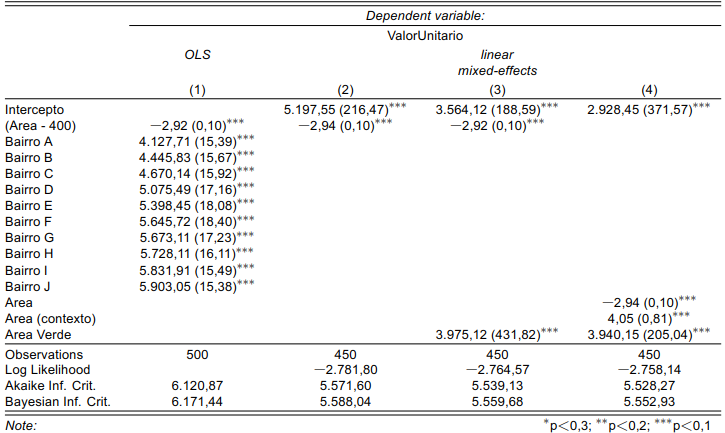
\includegraphics[width=0.8\linewidth]{../../images/tabela} \end{center}

\end{frame}

\begin{frame}{Modas Condicionais}
\protect\hypertarget{modas-condicionais}{}

\begin{itemize}[<+->]
\tightlist
\item
  Para o modelo misto simples, a variação não-explicada \emph{entre} os
  agrupamentos é alta!
\end{itemize}

\begin{figure}

{\centering 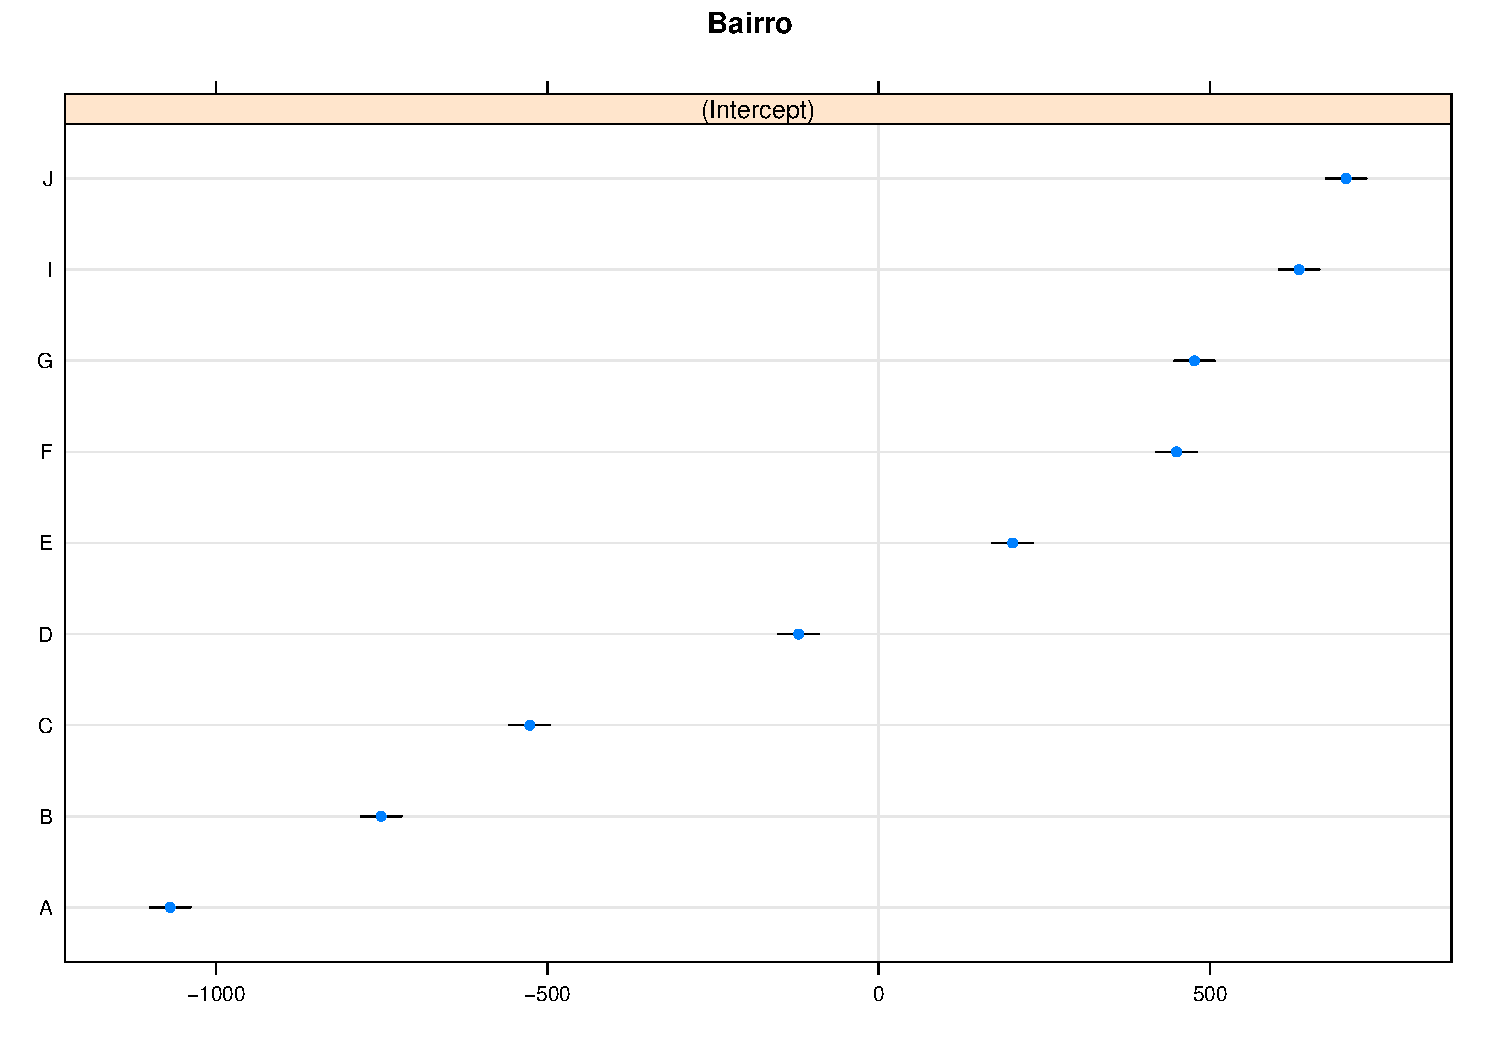
\includegraphics[width=0.6\linewidth]{index_files/figure-beamer/unnamed-chunk-10-1} 

}

\caption{Modas Condicionais do modelo misto simples.}\label{fig:unnamed-chunk-10}
\end{figure}

\end{frame}

\begin{frame}{Modas Condicionais}
\protect\hypertarget{modas-condicionais-1}{}

\begin{itemize}[<+->]
\tightlist
\item
  Com variáveis de segundo nível, a variação não-explicada \emph{entre}
  os agrupamentos é reduzida!
\end{itemize}

\begin{figure}

{\centering 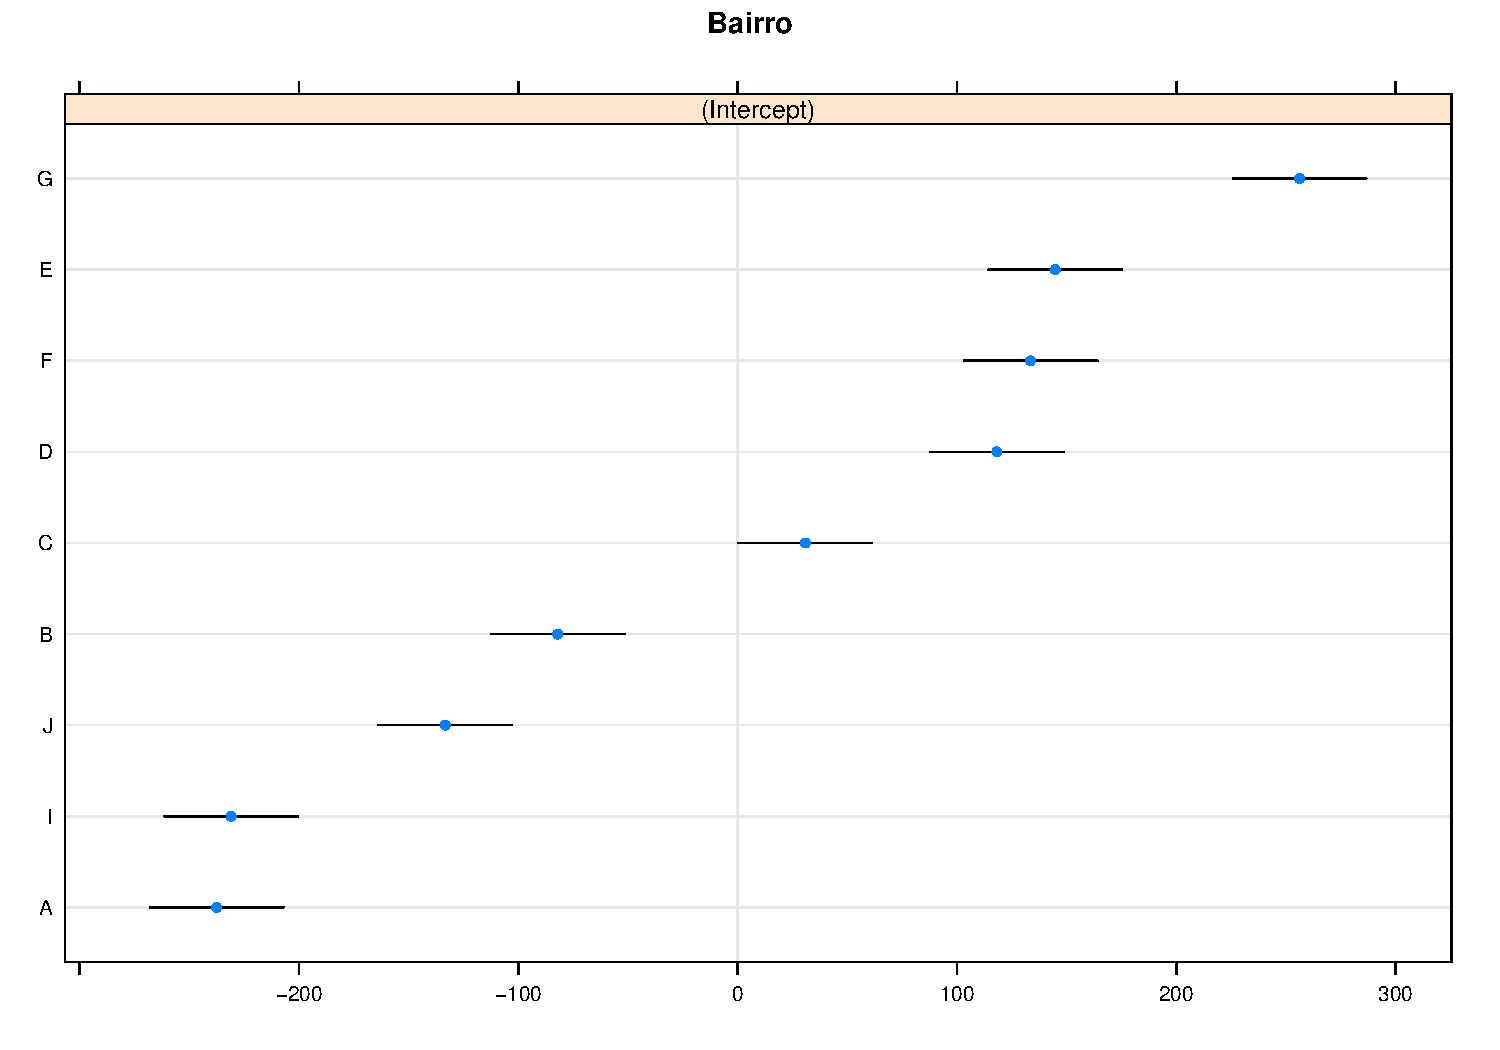
\includegraphics[width=0.6\linewidth]{index_files/figure-beamer/unnamed-chunk-11-1} 

}

\caption{Modas Condicionais do modelo misto com variável de 2º nível.}\label{fig:unnamed-chunk-11}
\end{figure}

\end{frame}

\begin{frame}{Modas Condicionais}
\protect\hypertarget{modas-condicionais-2}{}

\begin{itemize}[<+->]
\tightlist
\item
  Com a formulação de Mundlak, a variação não-explicada \emph{entre} os
  agrupamentos é reduzida ainda mais!
\end{itemize}

\begin{figure}

{\centering 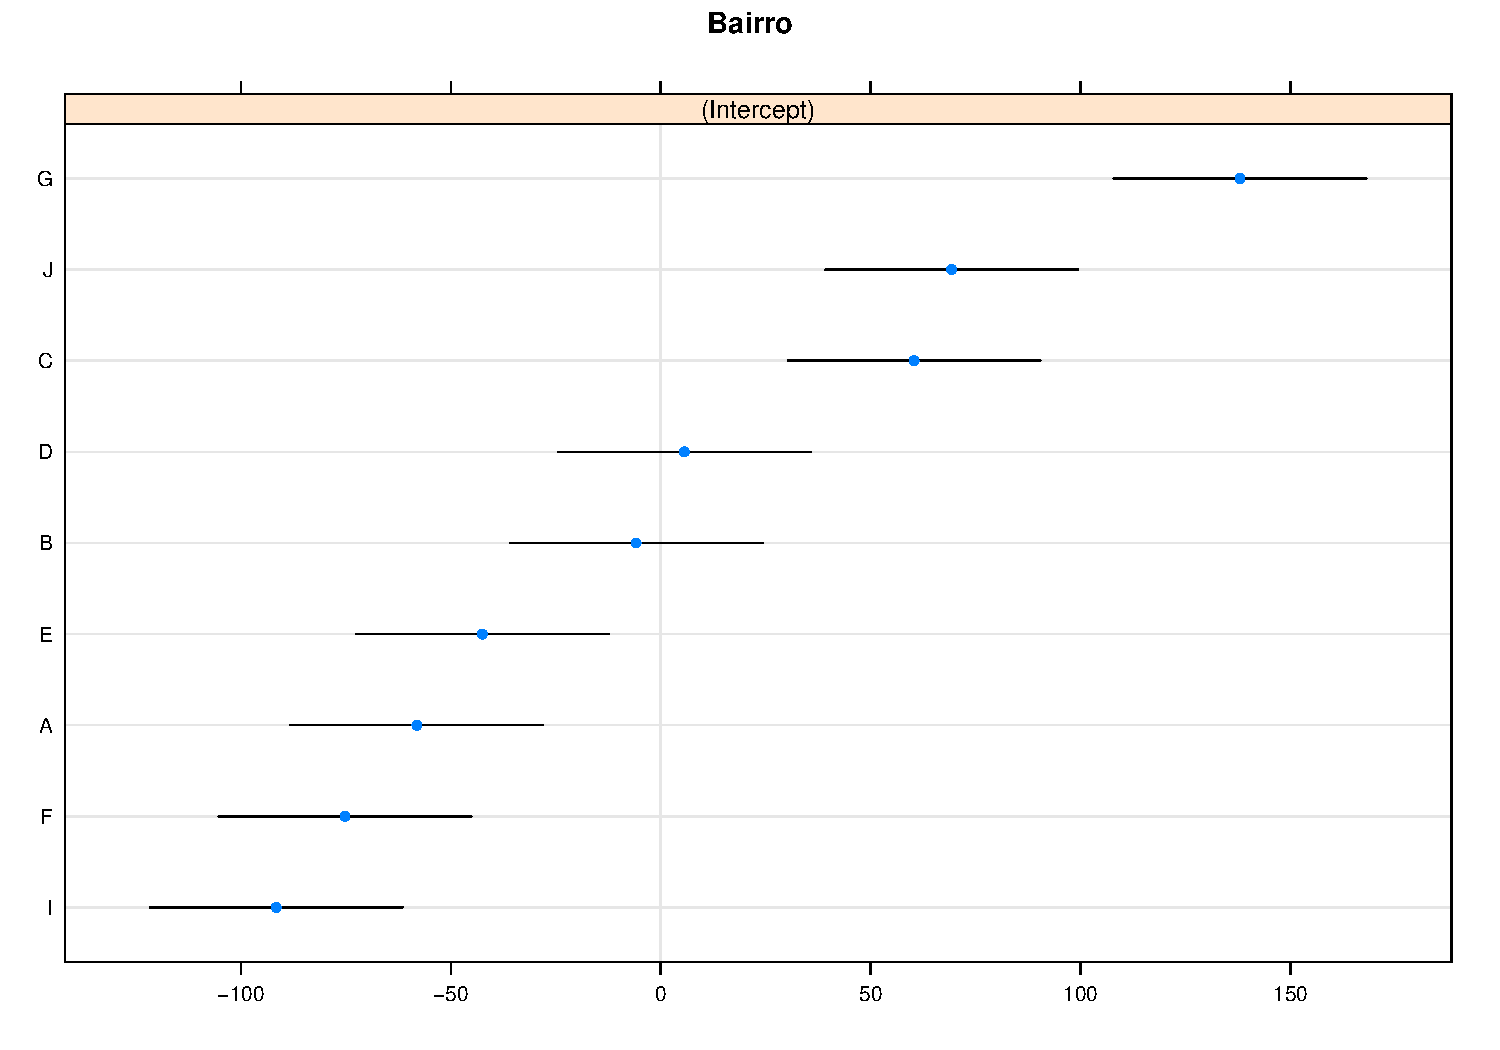
\includegraphics[width=0.6\linewidth]{index_files/figure-beamer/unnamed-chunk-12-1} 

}

\caption{Modas Condicionais do modelo misto com variável de 2º nível.}\label{fig:unnamed-chunk-12}
\end{figure}

\end{frame}

\begin{frame}{Densidade dos parâmetros estimados}
\protect\hypertarget{densidade-dos-paruxe2metros-estimados}{}

\begin{itemize}[<+->]
\tightlist
\item
  Para o modelo misto simples, a variação não-explicada \emph{entre} os
  agrupamentos (\(\sigma_1\)) é alta!
\end{itemize}

\begin{figure}

{\centering 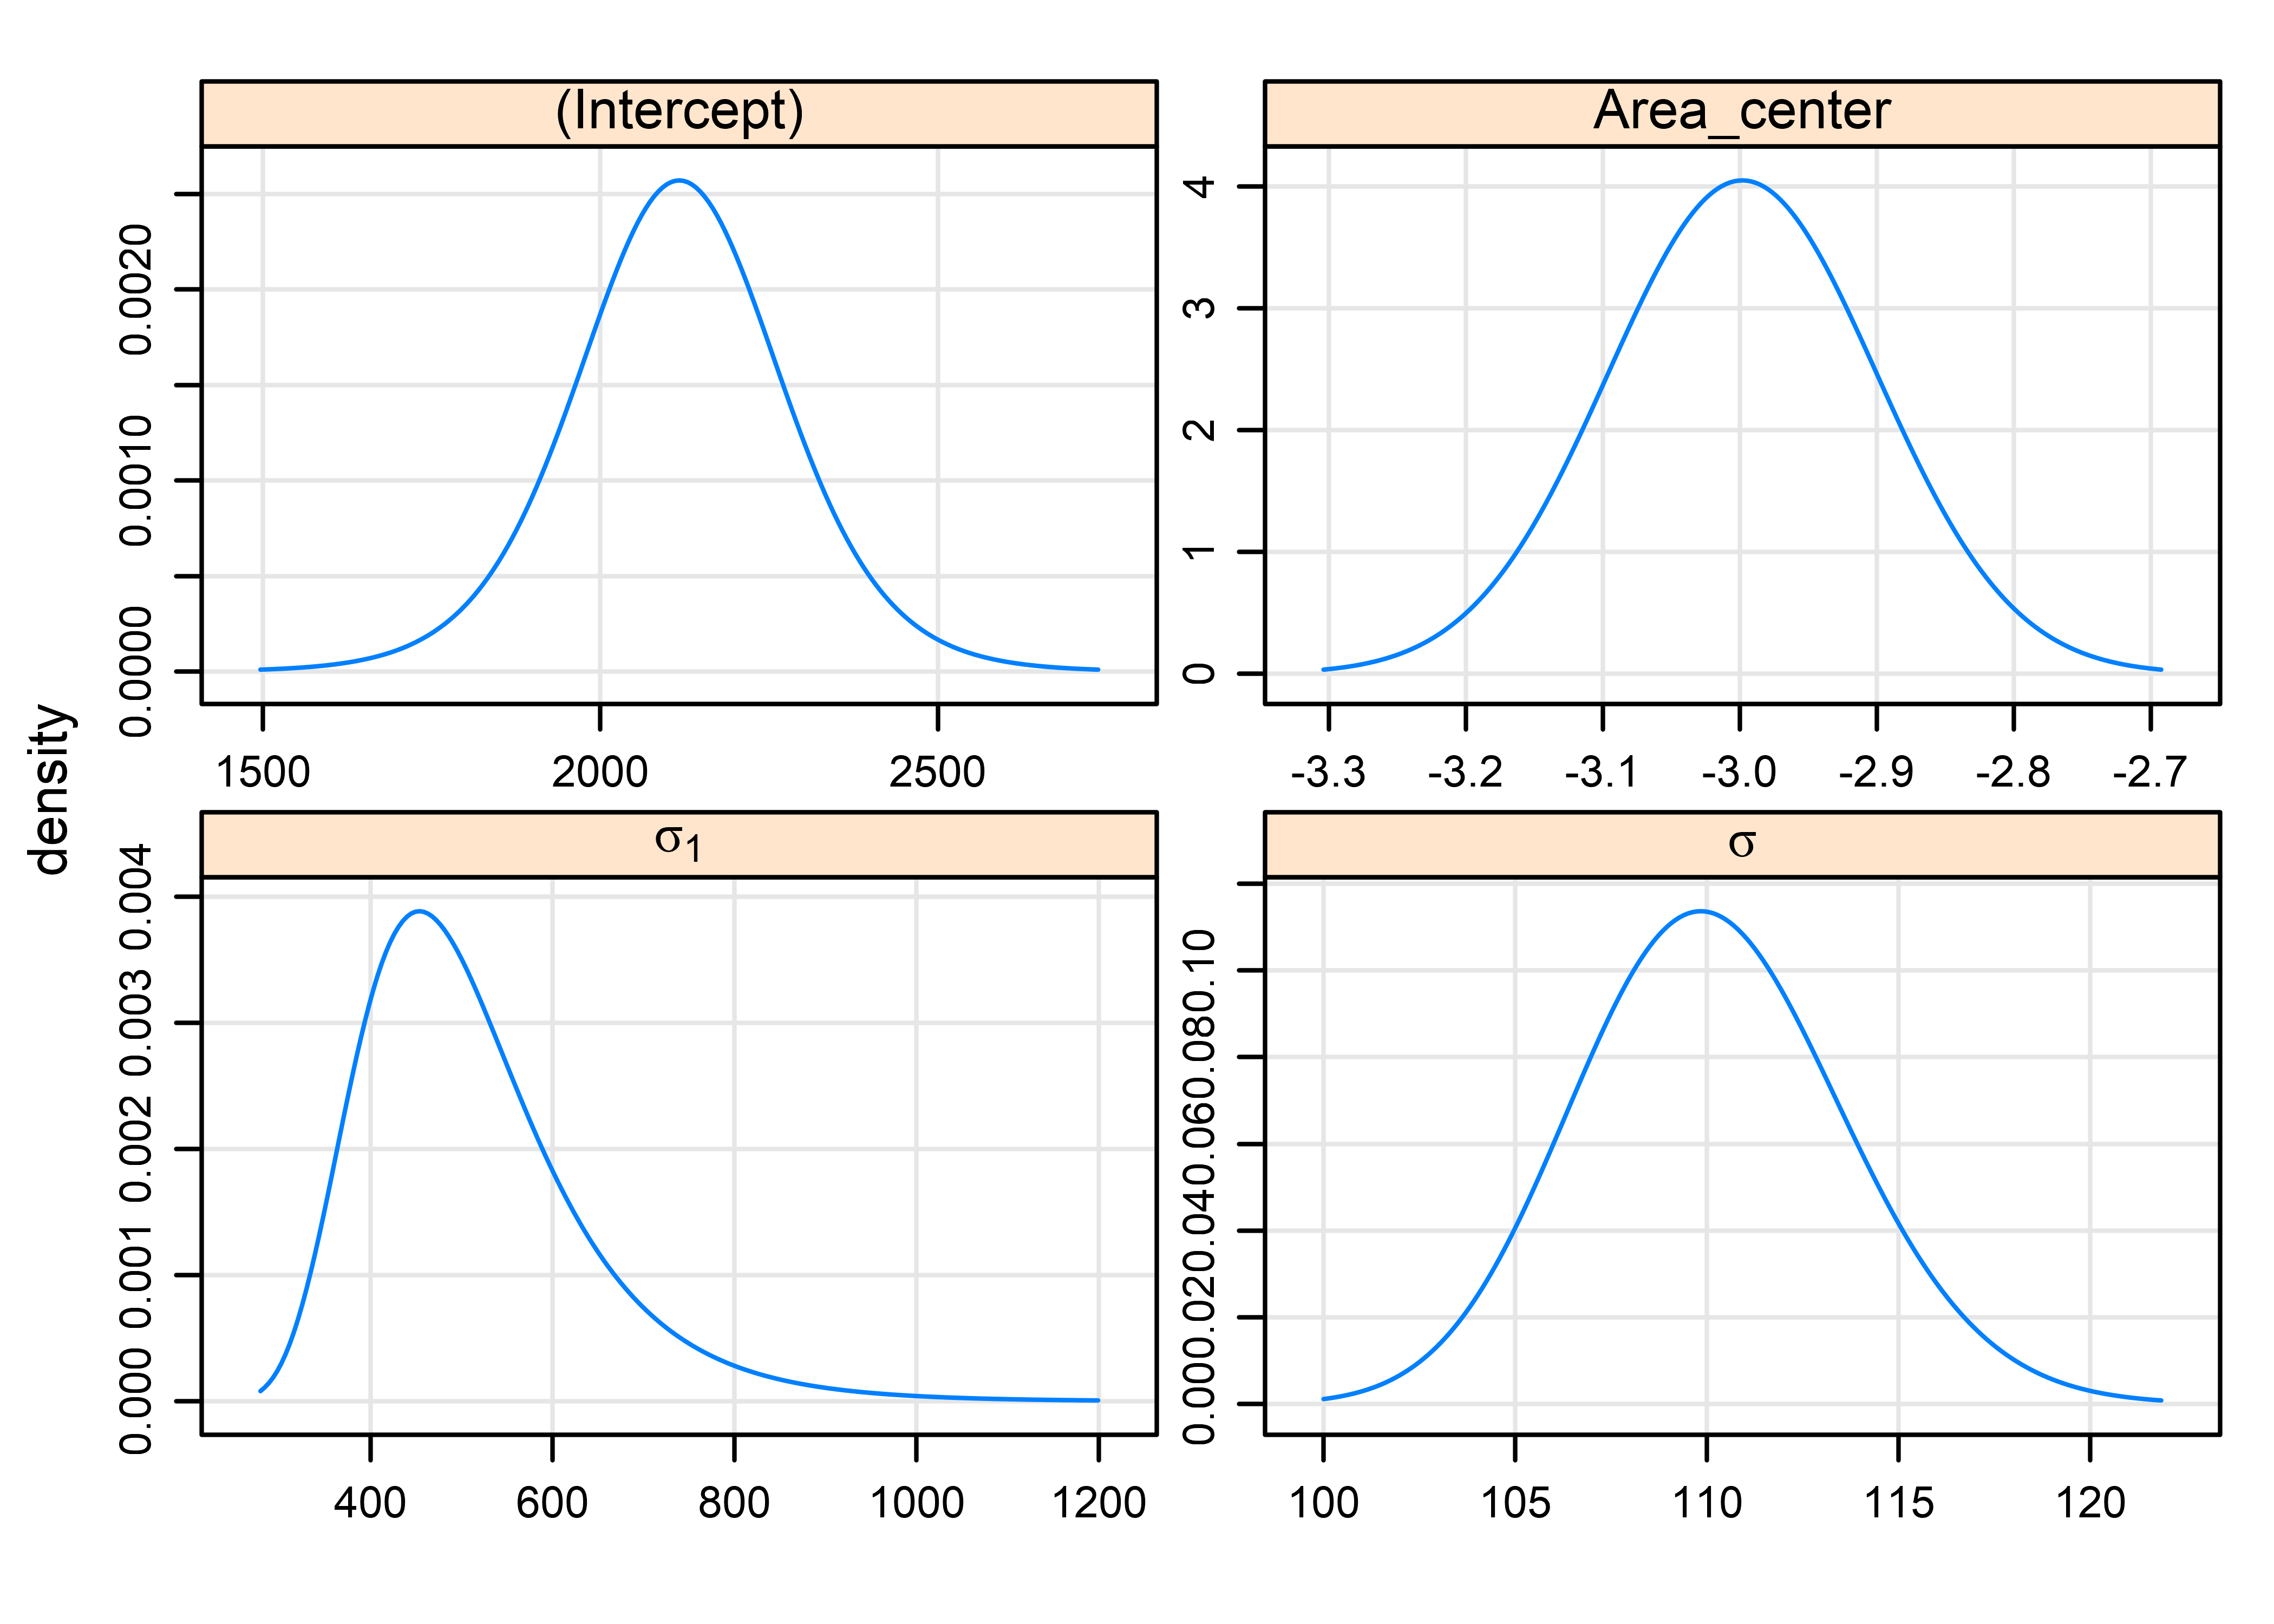
\includegraphics[width=0.4\linewidth]{../../images/pr-1} 

}

\caption{Densidades dos parâmetros estimados pelo modelo misto simples.}\label{fig:unnamed-chunk-13}
\end{figure}

\end{frame}

\begin{frame}{Densidade dos parâmetros estimados}
\protect\hypertarget{densidade-dos-paruxe2metros-estimados-1}{}

\begin{itemize}[<+->]
\tightlist
\item
  Com a introdução de variáveis de segundo nível, há redução da variação
  não-explicada \emph{entre} os agrupamentos (\(\sigma_1\))!
\end{itemize}

\begin{figure}

{\centering 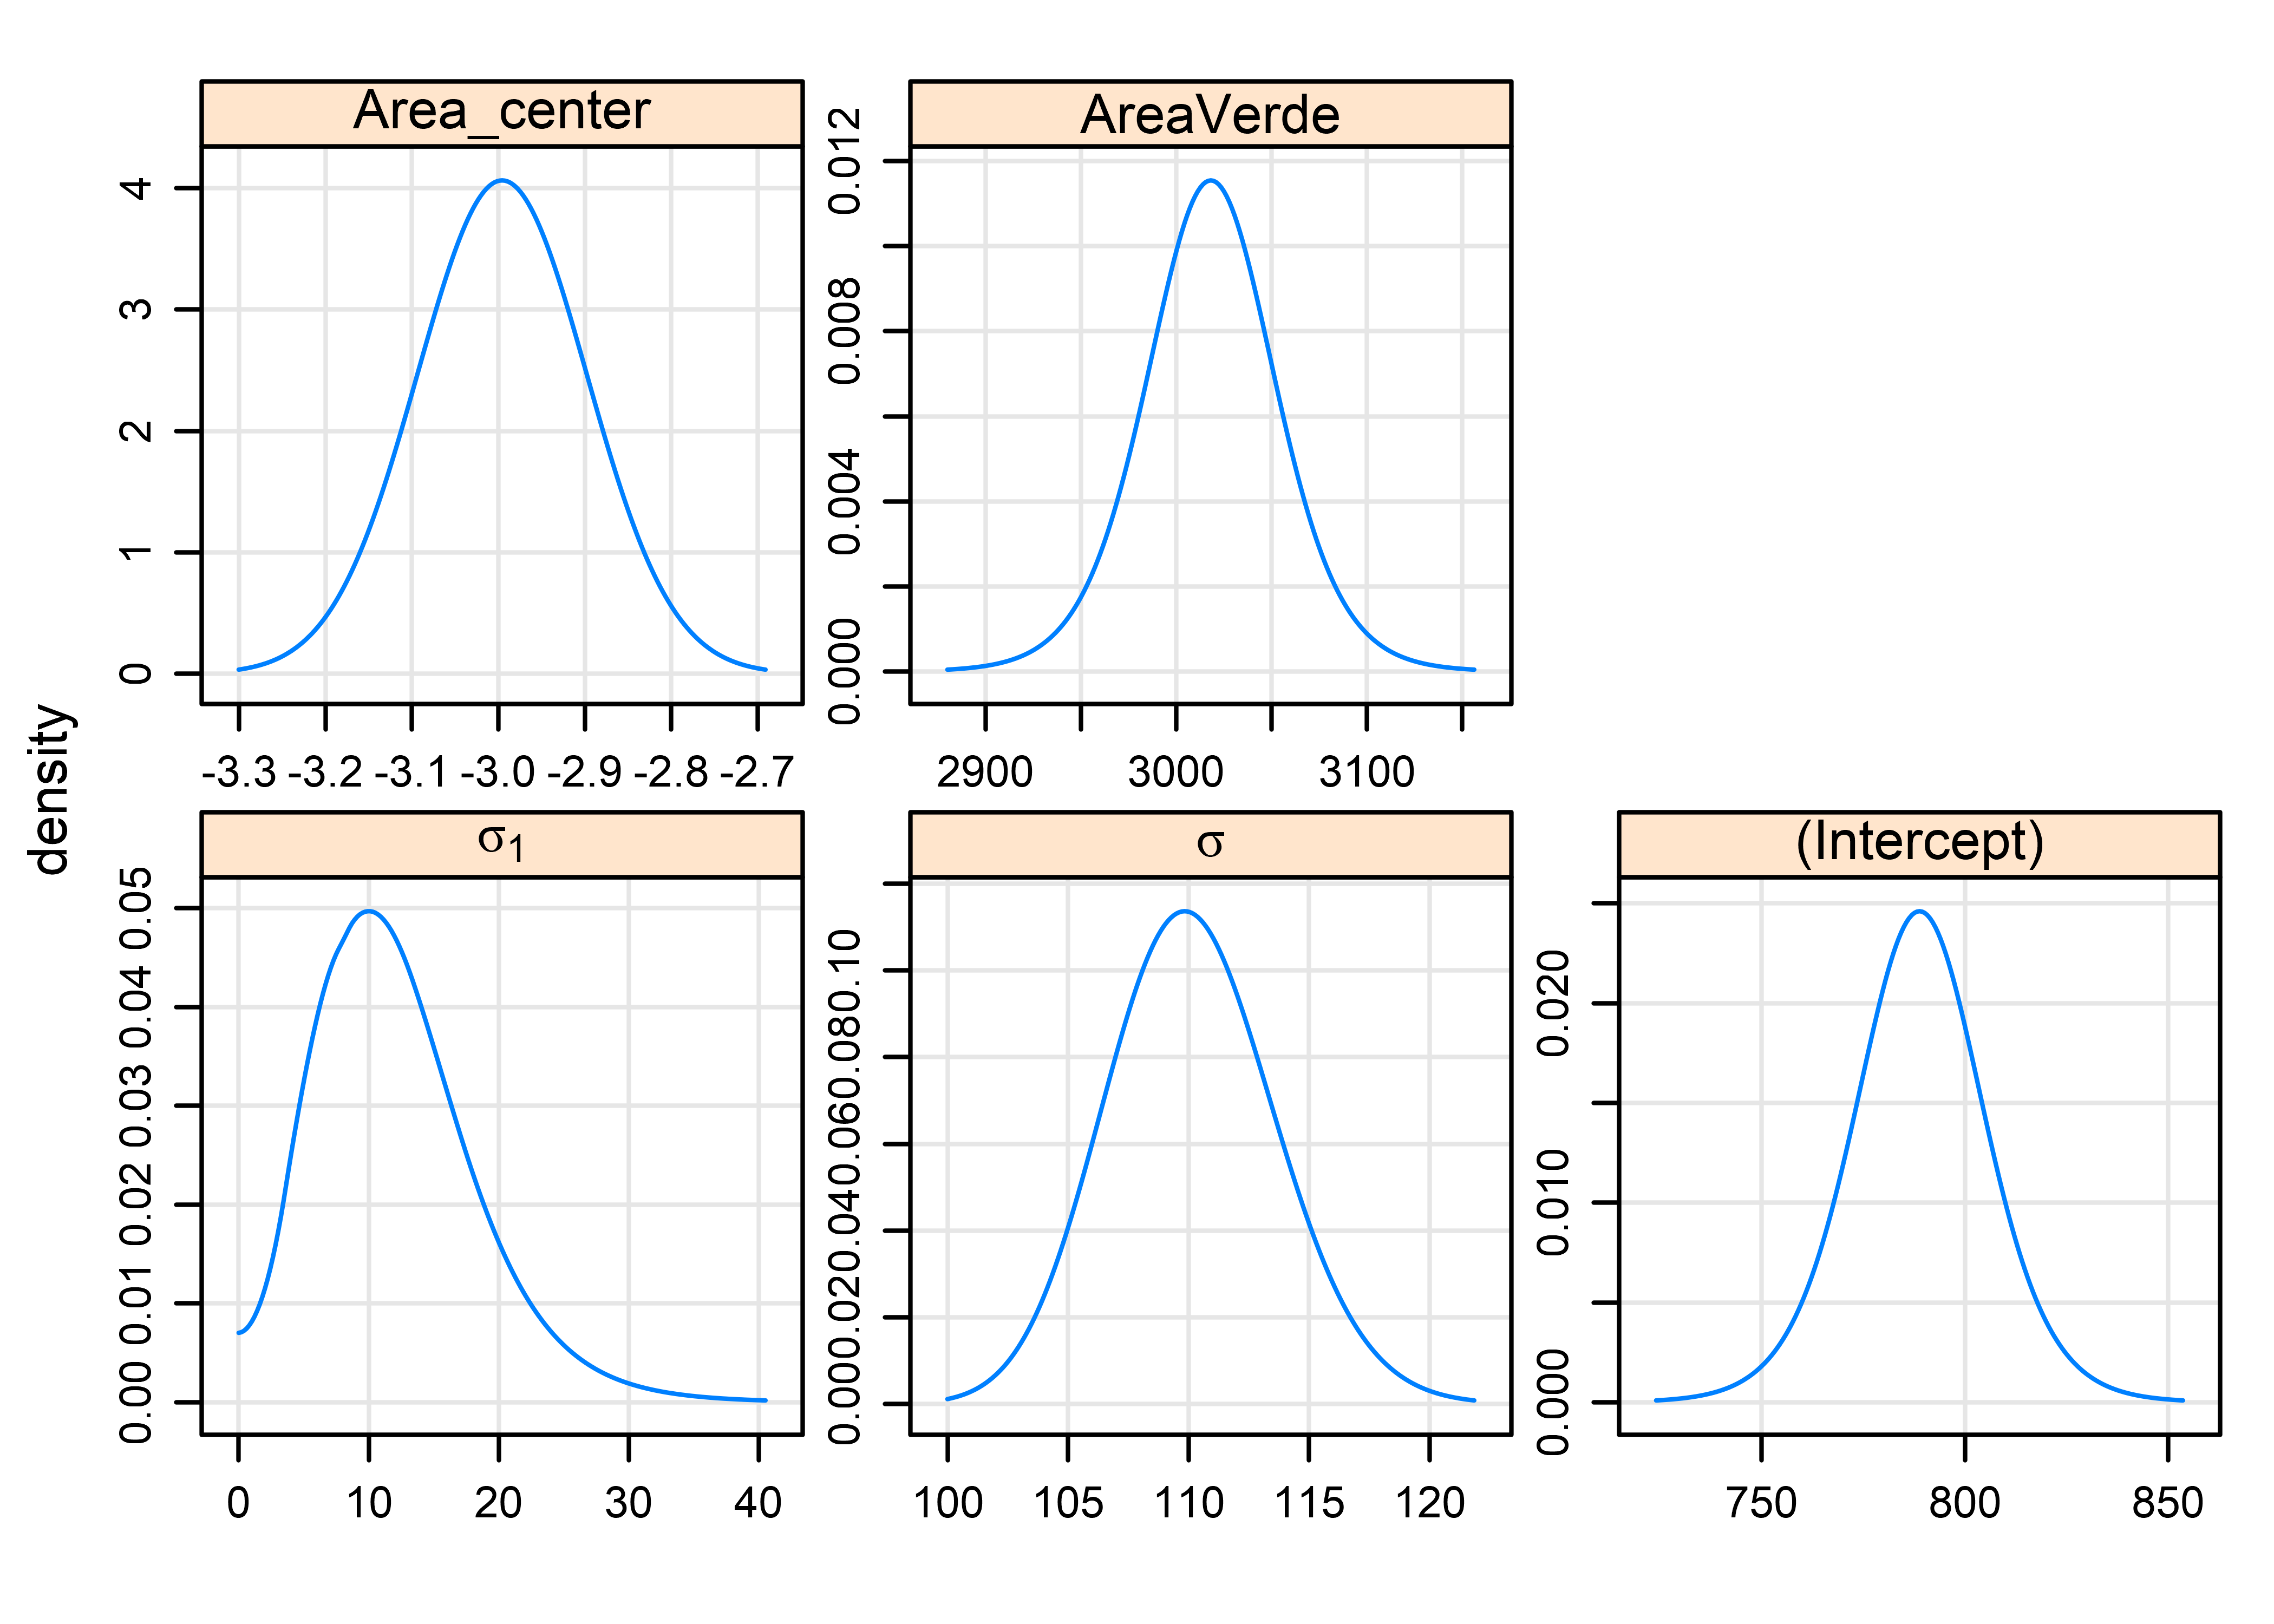
\includegraphics[width=0.5\linewidth]{../../images/pr1-1} 

}

\caption{Densidades dos parâmetros estimados pelo modelo misto com variável de 2º nível.}\label{fig:unnamed-chunk-14}
\end{figure}

\end{frame}

\begin{frame}{Densidade dos parâmetros estimados}
\protect\hypertarget{densidade-dos-paruxe2metros-estimados-2}{}

\begin{itemize}[<+->]
\tightlist
\item
  Com a formulação de Mundlak, há redução ainda maior da variação
  não-explicada \emph{entre} os agrupamentos (\(\sigma_1\))!
\end{itemize}

\begin{figure}

{\centering 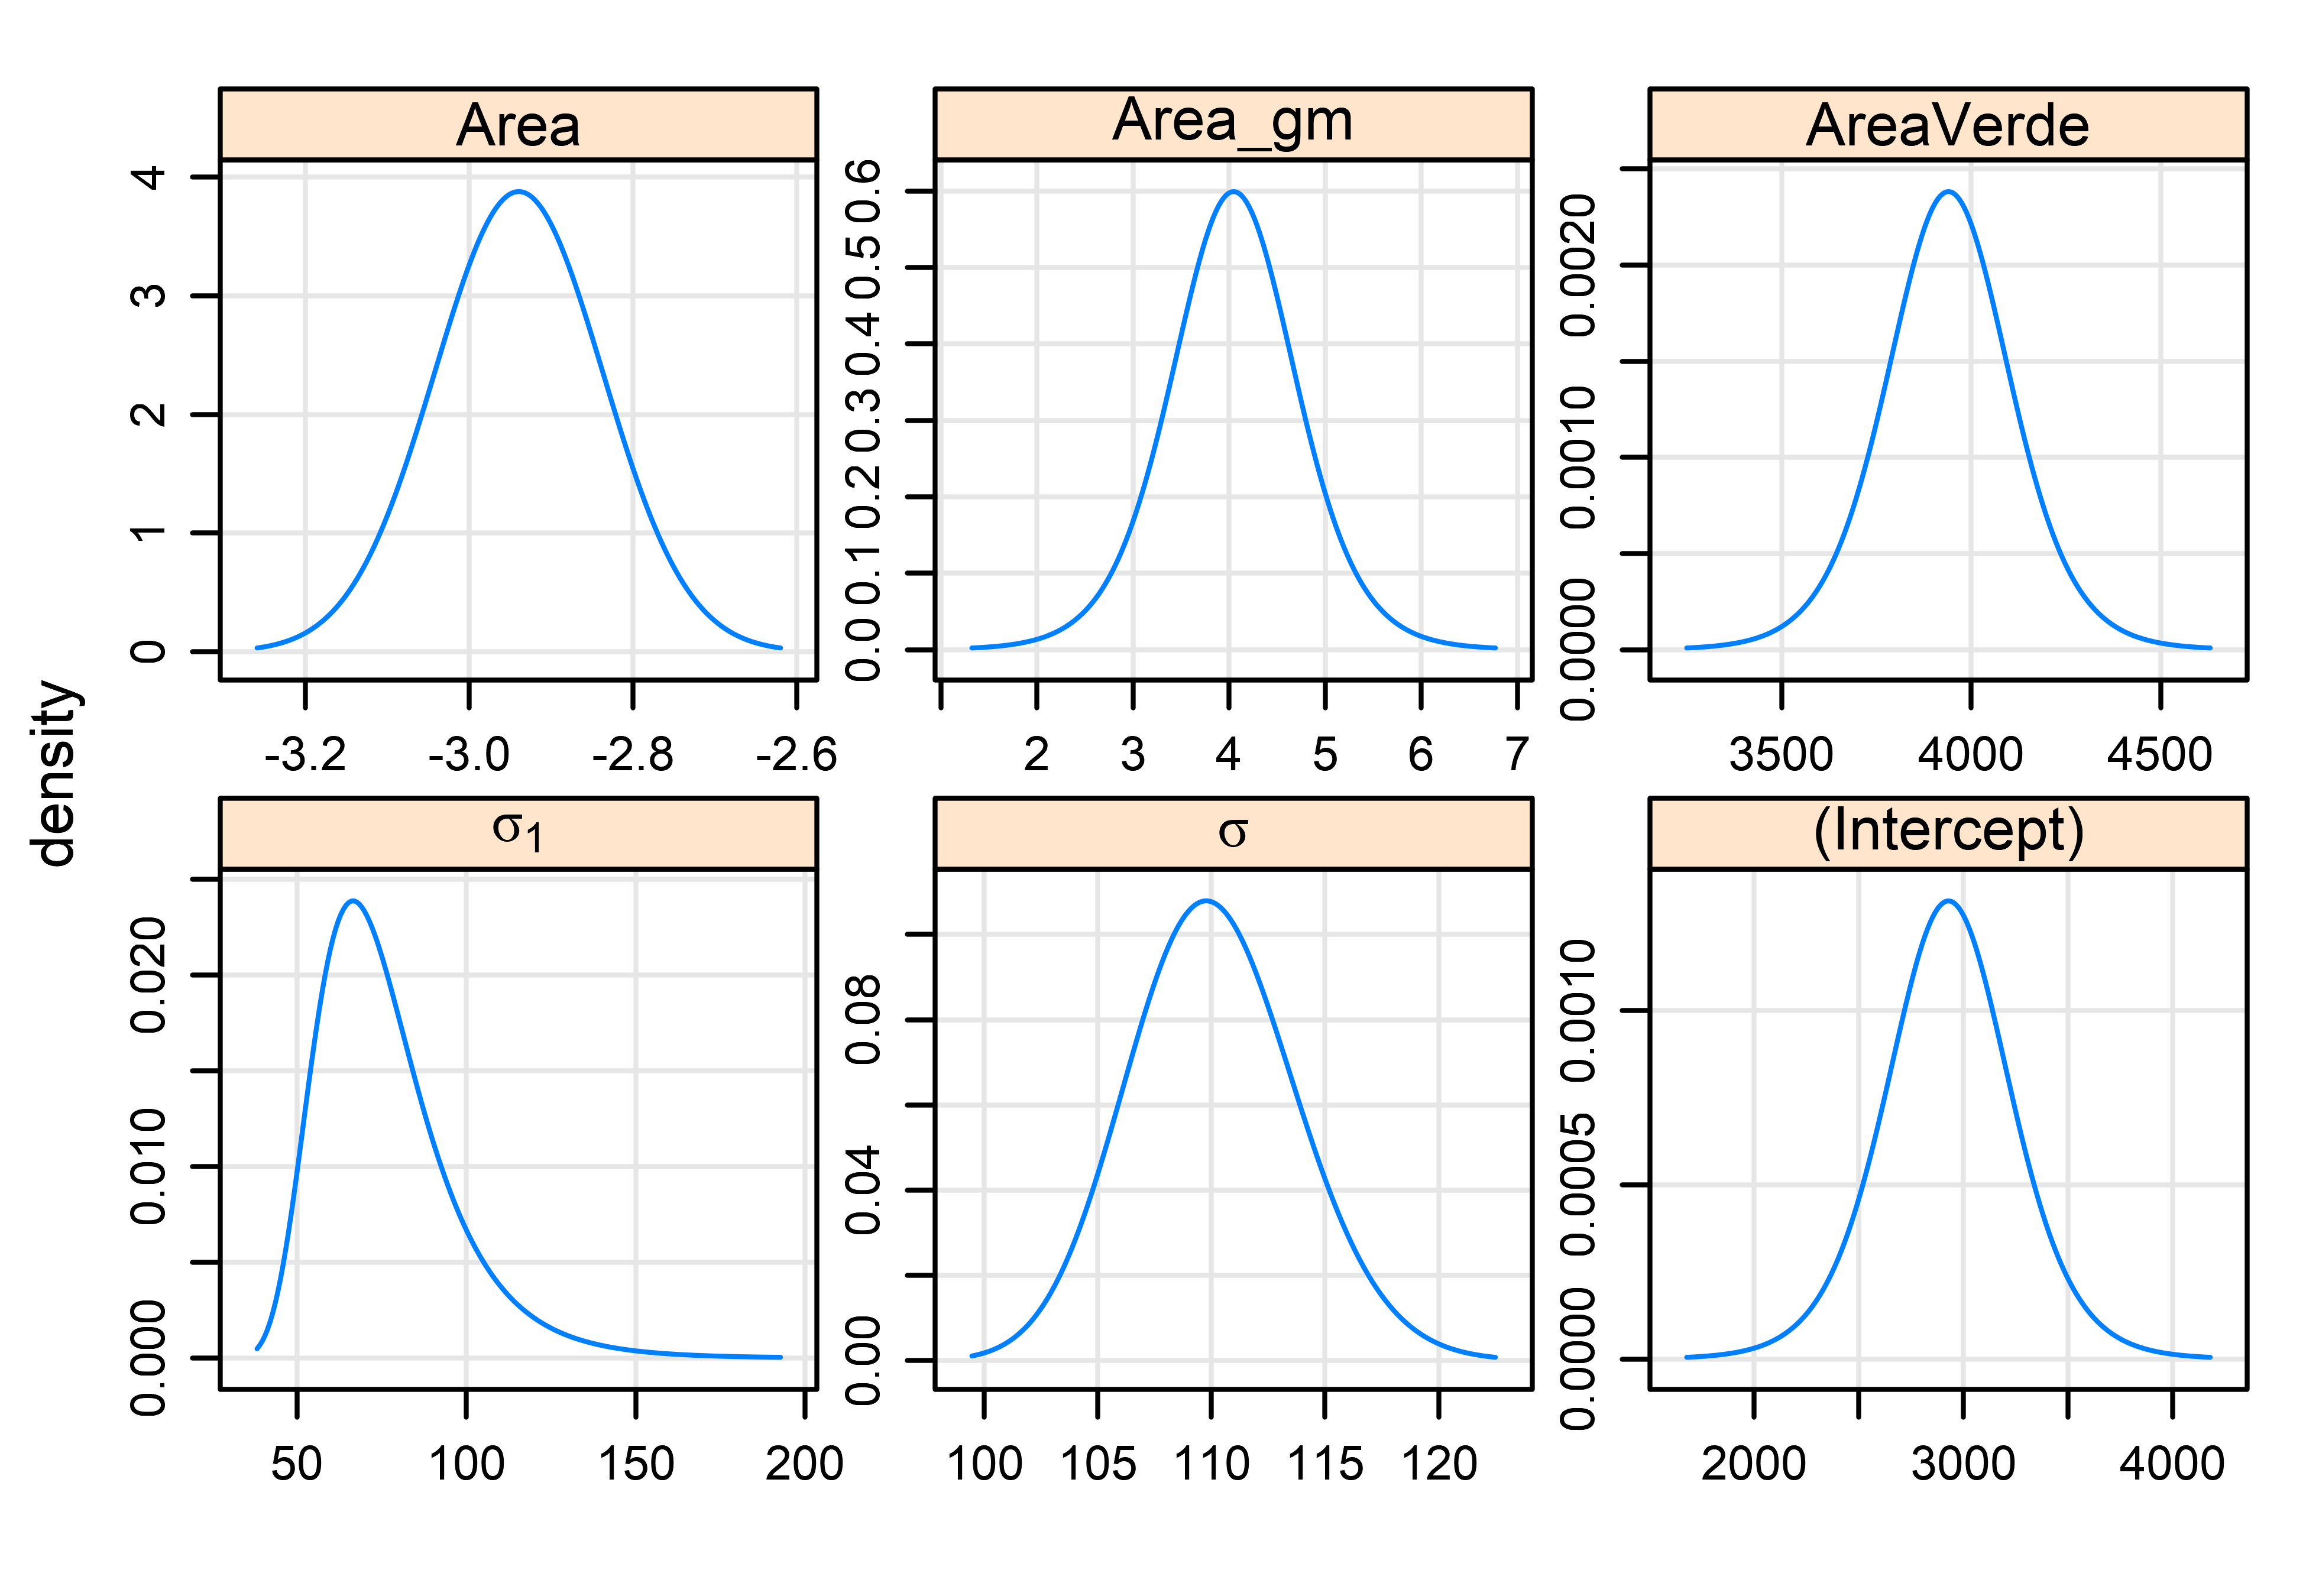
\includegraphics[width=0.5\linewidth]{../../images/pr2-1} 

}

\caption{Densidades dos parâmetros estimados pelo modelo com formulação de Mundlak.}\label{fig:unnamed-chunk-15}
\end{figure}

\end{frame}

\begin{frame}{Previsão de valores}
\protect\hypertarget{previsuxe3o-de-valores}{}

\begin{itemize}[<+->]
\tightlist
\item
  Modelos com variáveis de segundo nível capazes de prever valores em
  agrupamentos fora da amostra!
\end{itemize}

\begin{figure}

{\centering 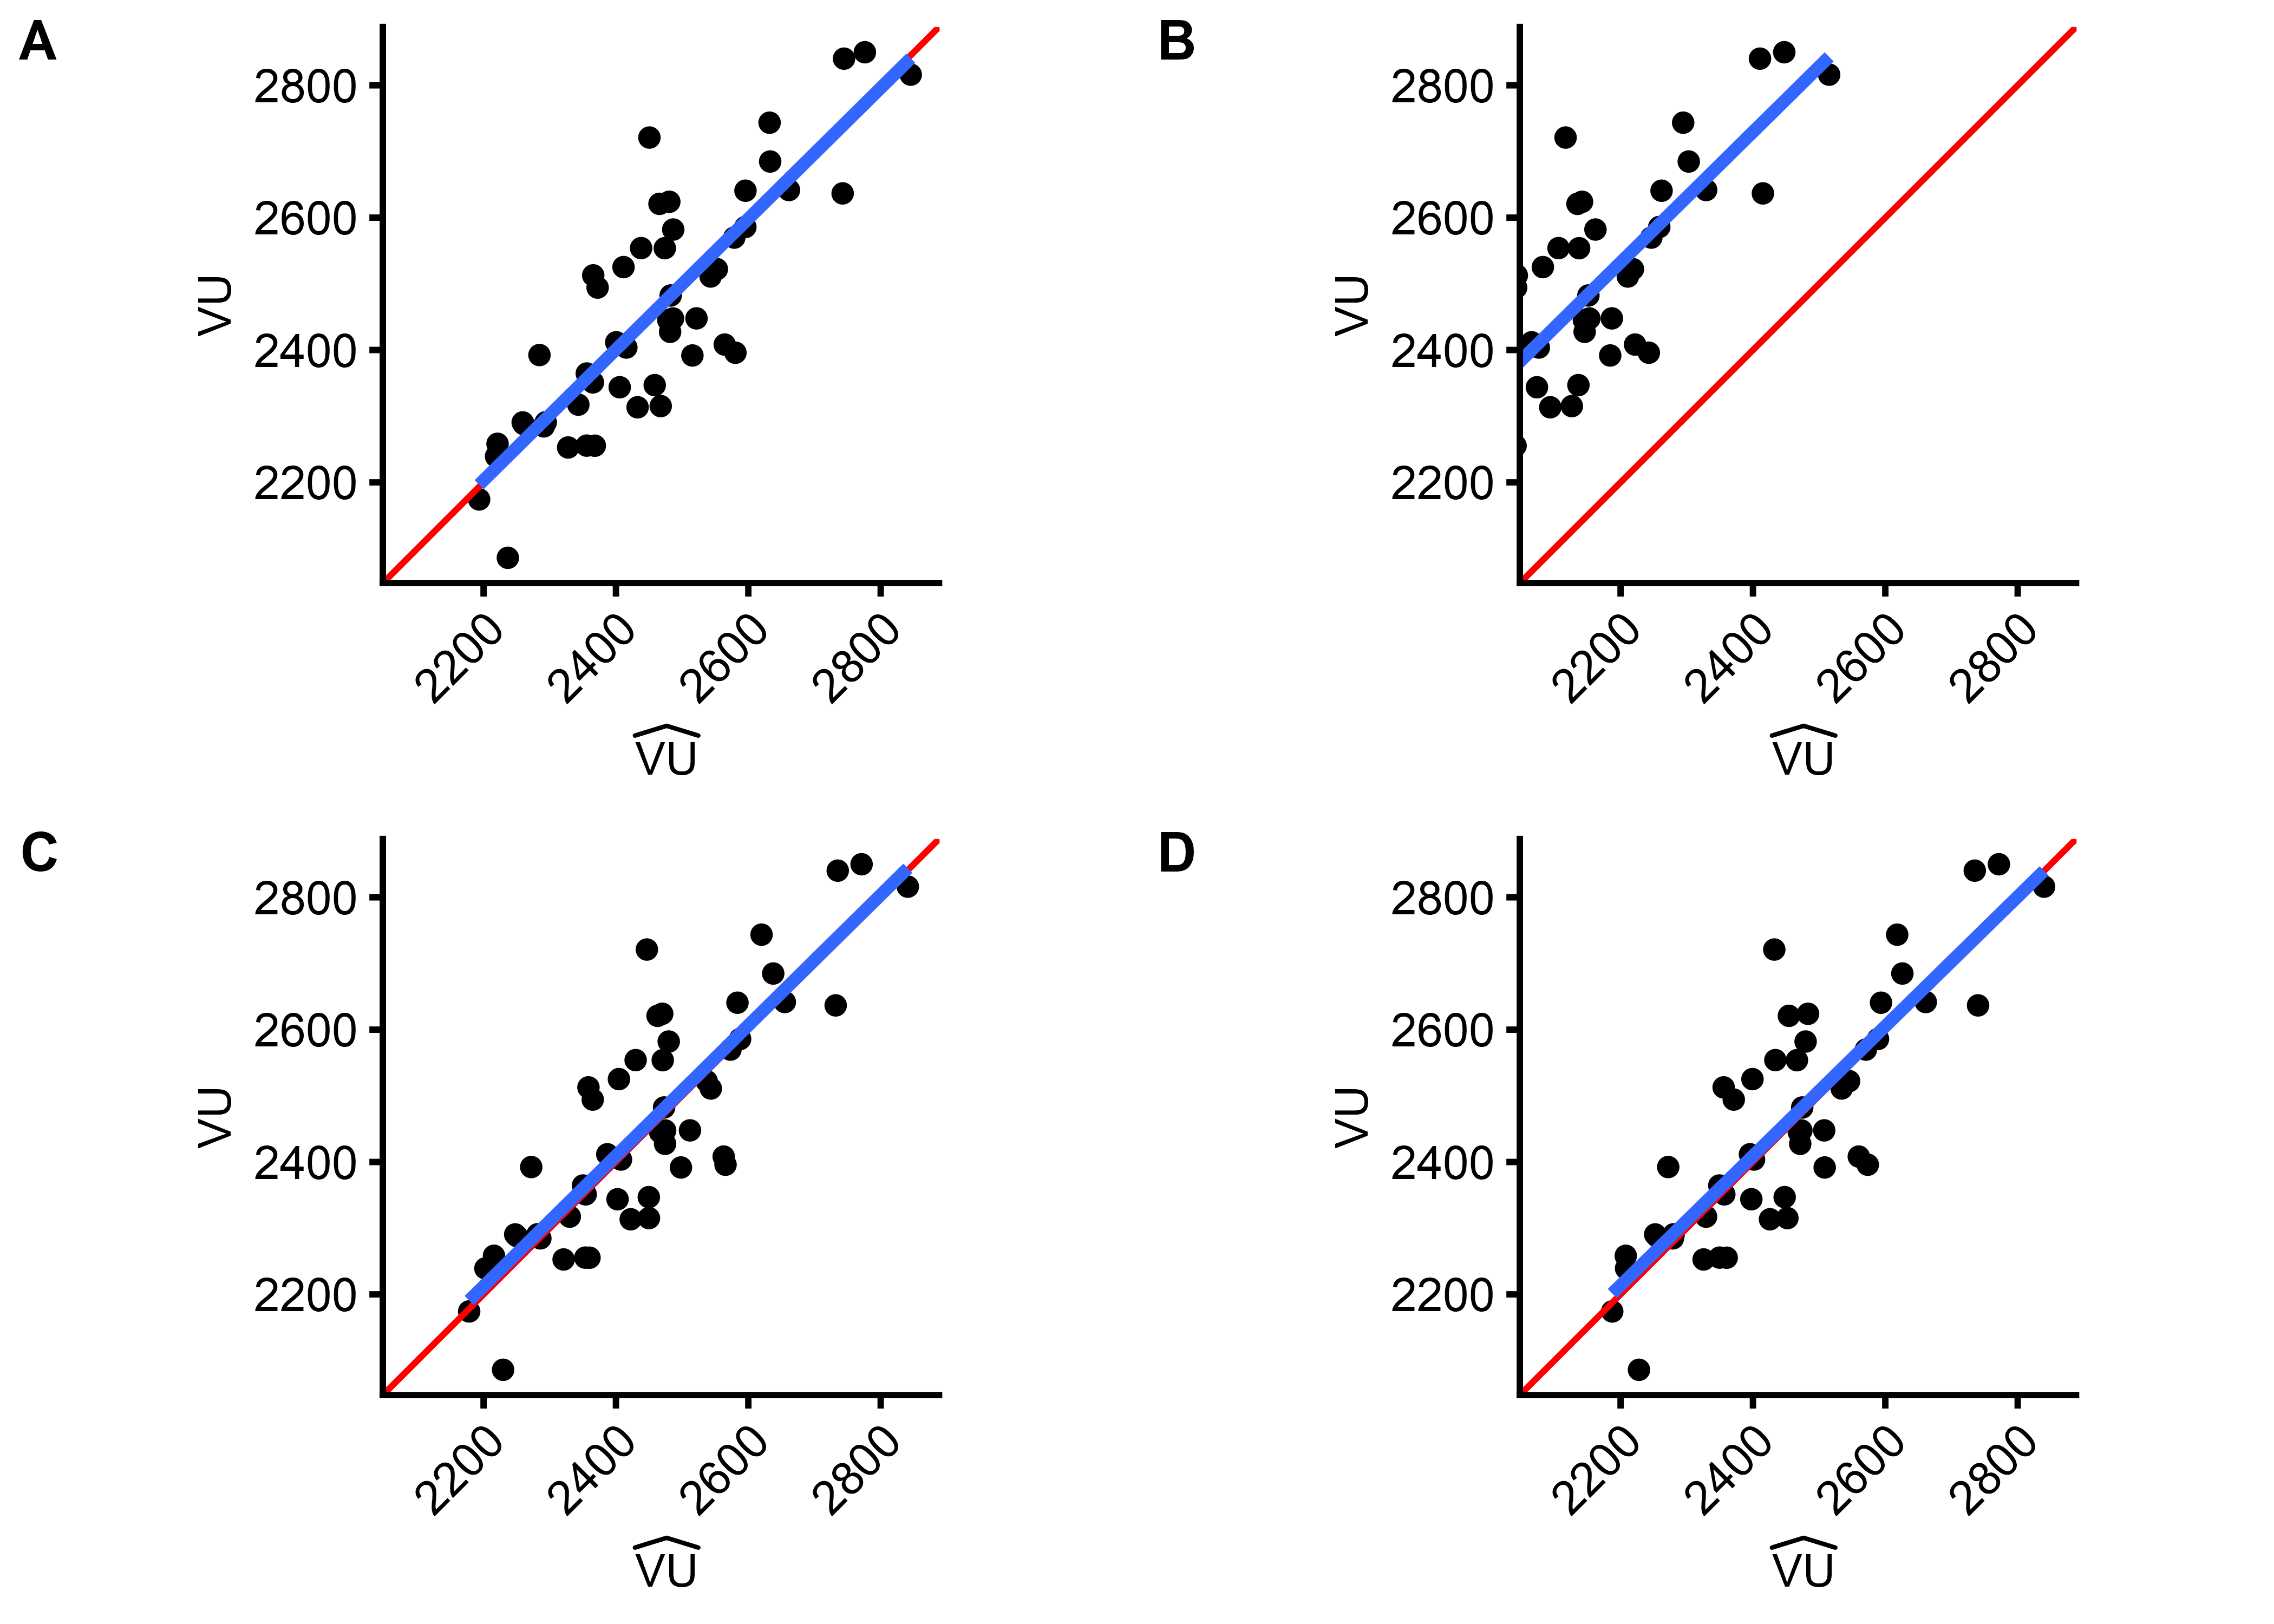
\includegraphics[width=0.5\linewidth]{../../images/powerPlots-1} 

}

\caption{Poder de predição para o bairro H em diversos modelos. Fonte: Os autores.}\label{fig:unnamed-chunk-16}
\end{figure}

\end{frame}

\begin{frame}{Intervalos de Predição}
\protect\hypertarget{intervalos-de-prediuxe7uxe3o}{}

\begin{center}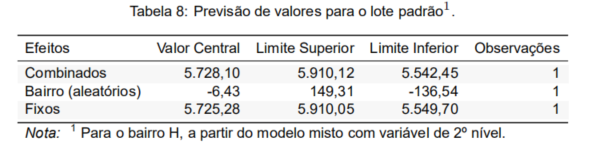
\includegraphics[width=0.5\linewidth]{tabela8} \end{center}

\begin{center}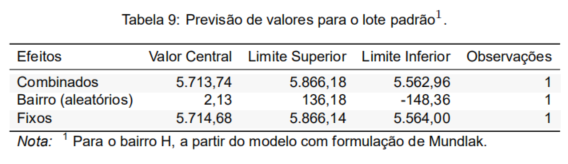
\includegraphics[width=0.5\linewidth]{tabela9} \end{center}

\begin{center}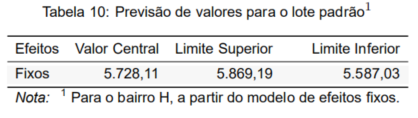
\includegraphics[width=0.5\linewidth]{tabela10} \end{center}

\end{frame}

\hypertarget{conclusuxf5es}{%
\section{Conclusões}\label{conclusuxf5es}}

\begin{frame}{Conclusões}

\begin{itemize}[<+->]
\tightlist
\item
  \alert<1>{Os modelos mistos podem ter importantes aplicações na Engenharia de
  Avaliações, desde que seja adotada a formulação adequada}

  \begin{itemize}[<+->]
  \tightlist
  \item
    \alert<2>{Nos laudos de precisão, devido ao \emph{borrowing strenght}}
  \item
    \alert<3>{Na avaliação em massa, devido ao alto número de diferentes
    agrupamentos e à facilidade para modelagem de inclinações aleatórias}
  \item
    \alert<4>{Na previsão do valor do solo em áreas adensadas, devido à 
    possibilidade de previsão de valores em agrupamentos fora da amostra}
  \item
    \alert<5>{Na análise de dados em séries temporais ou em painel, devido à
    possibilidade de separação dos efeitos \emph{dentro} e \emph{entre} os 
    agrupamentos (REWB)}
  \item
    \alert<6>{Na confecção de índices de preços}
  \end{itemize}
\end{itemize}

\end{frame}

\hypertarget{trabalhos-futuros}{%
\section{Trabalhos Futuros}\label{trabalhos-futuros}}

\begin{frame}{Modelagem de diversos níveis hierárquicos}
\protect\hypertarget{modelagem-de-diversos-nuxedveis-hieruxe1rquicos}{}

\begin{align*}
VU_{ijk}  &= \beta_{0jk} + \beta_{1jk} V_{1ijk} + \beta_{2jk} V_{2ijk} + \cdots + r_{ijk}\\ 
\beta_{0jk} &= \gamma_{00k} + \gamma_{01k}W_{1jk} + \gamma_{02k}W_{2jk} + \cdots+ s_{0jk}\\ 
\beta_{1jk} &= \gamma_{10k} + \gamma_{11k}W_{1jk} + \gamma_{12k}W_{2jk} + \cdots+ s_{1jk}\\ 
\vdots \\
\gamma_{00k} &= \eta_{000} + \eta_{001} X_{1k} + \eta_{002} X_{2k} + \cdots +  t_{00k}\\ 
\gamma_{01k} &= \eta_{010} + \eta_{011} X_{1k} + \eta_{012} X_{2k} + \cdots +  t_{01k}\\ 
\vdots
\end{align*}

\end{frame}


  \begin{frame}[allowframebreaks]{Referências}
  \bibliographytrue
  \printbibliography[heading=none]
  \end{frame}


\end{document}
